\documentclass{beamer}

\usepackage[utf8]{inputenc}
\usepackage[T1]{fontenc}
\usepackage[french]{babel}
\usepackage[ddmmyyyy]{datetime}

\usetheme{Warsaw}
\useinnertheme{rectangles}
\setbeamerfont{headline}{size=\large}
\setbeamerfont{frametitle}{size=\normalsize}

%Plan/Sommaire automatique avant chaque section
\AtBeginSection[]{
  \begin{frame}
  \frametitle{Plan}
  \tableofcontents[currentsection]
  \end{frame}
}

\author{Sonny Klotz - Jean-Didier Pailleux - Malek Zemni}
\institute{UVSQ}
\date{\today}
\usepackage{../tex/myInfolines}
\usepackage{longtable,array}
\title{Présentation Cahier des Charges}

\begin{document}

	\begin{frame}
		\titlepage
	\end{frame}
	
	\begin{frame}
		\frametitle{Plan général}
		\tableofcontents
	\end{frame}
	
	\section{Introduction}
	\begin{frame}
		Malek
	\end{frame}
	
	\section{Motivations}
	\begin{frame}
		Malek
	\end{frame}	
	
	\section{Contraintes}
	\begin{frame}
		Malek
	\end{frame}
	
	\section{Exigences fonctionnelles}
	\begin{frame}
		Sonny
	\end{frame}
	
	\section{Exigences fonctionnelles}
	\begin{frame}
		\begin{center}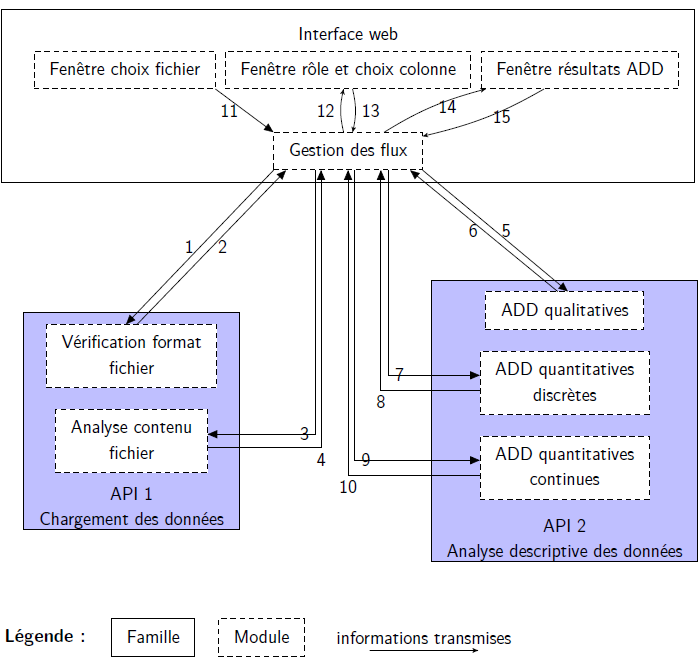
\includegraphics[scale=0.43]{org.png}\end{center}
	\end{frame}
	
	\section{Exigences non fonctionnelles}
	\begin{frame}
		Jean-Édouard
	\end{frame}
	
	\section{Autres aspects}
	\begin{frame}
		\begin{itemize}
		\item \textbf{Question ouverte} : Esthétisme et présentation des résultats laissé ouverte. Approche prenant en compte les utilisateurs.
		\item \textbf{Choix du langage} :
		\item \textbf{Tâche à faire} :
		\item \textbf{Contrôle de la finalisation} :
		\item \textbf{Estimation des coûts} : Une estimation de 565 lignes de code.
		\item \textbf{Documentation utilisateur et formation} : Pas de formation, mais documentation fournie.
		\item \textbf{Répartition des tâches} : 
		\begin{center}\begin{longtable}{|>{\centering}m{5cm}|>{\centering}m{2cm}|>{\centering}m{2cm}|>{\centering}m{2.5cm}|>{\centering\arraybackslash}m{1cm}|}			
			\hline \multicolumn{1}{|c|}{\textbf{Module}} & \multicolumn{1}{c|}{\textbf{Malek}} & \multicolumn{1}{ c|}{\textbf{Sonny}} & \multicolumn{1}{c|}{\textbf{Jean-Didier}} & {\textbf{Total}} \\
			\hline 	Gestion des flux & ~ & ~ & x & 1\\
			\hline 	Fenêtre choix fenêtre & ~ & ~ & x & 1\\
			\hline 	Fenêtre rôle et choix colonne & x & ~ & ~ & 1\\
			\hline 	Fenêtre résultats ADD & ~ & x & ~ & 1\\
			\hline  ADD qualitatives & ~ & ~ & x & 1\\
			\hline 	ADD quantitatives discrètes & ~ & x & ~ & 1\\
			\hline 	ADD quantitative continues &  ~ & x & ~ & 1\\
			\hline 	Vérification format fichier & x & ~ & ~ & 1\\
			\hline 	Analyse contenu fichier & x & ~ & ~ & 1\\
			\hline
			\end{longtable}\vspace{1em}\end{center}
		\end{itemize}
	\end{frame}
	
	\section{Conclusion}
	\begin{frame}
		Deux langages potentiels Java et Python. Notre choix s'est finalisé sur Python.
		\begin{itemize}
		\item \textbf{Python} : Langage préconisé par les startups pour construire des applications. 
		\item \textbf{Java} : Utilisé par les entreprises ayant les moyens pour le développement et la maintenance du système.
		\end{itemize}
		
		\textbf{Difficultés rencontrées :}  Apprendre une nouvelle démarche et pratique dans un projet à grande ampleur.\\
		
		
	\end{frame}
	
\end{document}
